\documentclass[a4paper,10pt]{report}
\usepackage{float,graphicx}
\usepackage{amsfonts}
\usepackage{amsthm}
\usepackage{amsmath}
\usepackage{amssymb}
\usepackage{wrapfig}
\usepackage{minted}
\usepackage{mathrsfs}
\usepackage{pgfplots}
\usepackage{mdframed}
\usepackage[lined,boxruled]{algorithm2e}\usepackage{color}
\usepackage[english]{babel}

\newcommand{\ac}[1]{\textcolor{red}{AC: #1}}
\newcommand{\af}[1]{\textcolor{blue}{AF: #1}}

\pgfplotsset{width=10cm,compat=1.9}
\usemintedstyle{friendly}
\BeforeBeginEnvironment{minted}{\begin{mdframed}}
\AfterEndEnvironment{minted}{\end{mdframed}}
\begin{document}
\title{\Large{\textbf{Inducing game rules from varying quality game play}}}
% \title{\Large{\textbf{Inductive general game playing with varying quality game play}}}
\author{Alastair Flynn}
\maketitle

\begin{abstract}

General Game Playing (GGP) is a framework in which an artificial intelligence program is required to play a variety of games successfully, it acts as a test bed for AI and motivator of research. The AI is given a random game description at runtime (such as checkers or tic tac toe) which it then plays.
The framework includes repositories of game rules written in a logic programming language.


The Inductive General Game Playing (IGGP) problem challenges machine learning systems to learn these GGP game rules by watching the game being played. In other words, IGGP is the problem of inducing general game rules from specific game observations. Inductive Logic Programming (ILP), a subsection of ML, has shown to be a promising approach to this problem though it has been demonstrated that it is still a hard problem for ILP systems. In this regard IGGP motivates future research in ILP.

Existing work on IGGP has always assumed that the game player being observed makes random moves. This is not representative of how a human learns to play a game, to learn to play chess we watch someone who is playing to win. With random gameplay a lot situation that would normally be encountered  when humans play are not present. It may be the case that some games rules do not come into effect unless the game gets to a certain state such as castling in checkers. Rules of games are designed with good play in mind so it would make sense that a good player of the game would invoke more cases of the rules.

To address this limitation, we analyse the effect of using intelligent verses random gameplay traces as well as the effect of varying the number of traces in the training set.

We use Sancho, the 2014 GGP competition winner, to generate optimal game traces for a large number of games.
We then use the ILP systems, Metagol, Aleph and ILASP to induce game rules from the traces.
We train and test the systems on combinations of intelligent and random data including a mixture of both. We also vary the volume of training data.

Our results show that whilst some games were learned more effectively in some of the experiments than others no overall trend was statistically significant. 

The implications of this work are that varying the quality of training data as described in this paper has strong effects on the accuracy of the learned game rules however one solution does not work for all games.




% When learning programs in Inductive Logic Programming (ILP) optimisations to the dataset used to train the systems can often be as effective as improvements to the systems themselves.


\end{abstract}

\chapter{Introduction}
General Game Playing (GGP) is a framework in which artificial intelligence programs are required to play a large number of games successfully.\cite{Genesereth/GGPOverview}. Traditional game playing AI has focused on a single game. Famouse AI such as IBMs deep blue is able to beat grand masters at chess but is completetly unable to play checkers \ac{citation needed}. These traditional AI also only do part of the work. A lot of the analysis of the game is done outside of the system. A more interesting challenge is building AI that can play games without any prior knowlegde. In GGP the AI are given the description of the rules of a game at runtime. Games in the framework range greatly in both number of players and complexity; from the single player Eight Puzzle to the six player Chinese Checkers, and from the relativly simple Rock Paper Scissors to Chess\cite{GGP-Website}. The progress in the field is consolidated annually at the GGP where participants compete to find the best GGP AI.

The GGP framework includes a large database of games. In a GGP match games from these databases are selected at random and sent to the competitors. The games are specified in the Game Description Language (GDL), a logic programming language built for describing games as state machines\cite{GDL_Spec}. A logic programming language being any that is mainly based on formal logic, such as Prolog.


\begin{figure}[ht]
	\centering
	\fbox{\includegraphics[width=0.7\linewidth]{GGP-Games.png}}
	\caption{A selection of games from the GGP competition. From the top right: \textit{checkers}, \textit{chinese checkers}, \textit{chess}, \textit{tic tac toe}, \textit{rubix cube} and \textit{eight puzzle}}
\end{figure}

\begin{listing}[ht]
\begin{minted}[fontsize=\footnotesize]{text}
(succ 0  1)
(succ 1  2)
(succ 2  3)
(beats scissors paper)
(beats paper stone)
(beats stone scissors)
(<= (legal ?p scissors) (player ?p))
(<= (legal ?p paper) (player ?p))
(<= (legal ?p stone) (player ?p))
(<= (draws ?p) (does ?p ?a) (does ?q ?a) (distinct ?p ?q))
(<= (wins ?p) (does ?p ?a1) (does ?q ?a2) (distinct ?p ?q) (beats ?a1 ?a2))
(<= (loses ?p) (does ?p ?a1) (does ?q ?a2) (distinct ?p ?q) (beats ?a2 ?a1))
\end{minted}
\caption{
\ac{is this listing referenced in the text?}
A sample of rules from the GDL description of Rock Paper Scissors. The $?$ indicates a variable and $<=$ indicates an implication with the first expression after being the head and the conjugation of the rest making up the body
}
\end{listing}


These GDL game descriptions form the basis for the Inductive General Game Playing (IGGP) problem \ac{citation needed}. The task is an inversion of the GGP problem. Rather than taking game rules and using them to play the game in IGGP the aim is to learn the rules from observations of gameplay, similar to how a human might work out the rules of a game by watching someone play it. Cropper et al. define the IGGP problem in their 2019 paper; given a set of gameplay observations the goal is to induce the rules of the game\cite{Cropper/IGGP}. The games used in IGGP are those from the GGP competition problem set, specified in GDL, meaning they are widely varied in complexity.

\af{GIVE EXAMPLE OF IGGP PROBLEM}

An effective way of solving the IGGP problem is a form of machine learning: Inductive Logic Programming (ILP) \ac{citation needed}. In ILP, the learner is tasked with learning logic programs given some background knowledge and a set of values for which the programs are true or false (also expressed in a logical programming language). In the IGGP paper \cite{Cropper/IGGP}, the authors showed through empirical evaluations that ILP systems achieve the best score in this task compared to other machine learning techniques. The ILP system derive a hypothesis, a logic program that when combined with the background knowledge, entails all of the positive and none of the negative examples\cite{Muggleton/ILP}. In the IGGP paper\cite{Cropper/IGGP} it is also shown that the problem is hard for current ILP systems, with on average only 40\% of the rules being learned by the best performing systems.

However, the existing work has limitations. All existing work has assumed that the gameplay being observed is randomly generated. Rather than agents playing to win they simply make moves at random. Often this has the result of the game terminating before it reaches a terminal state due to a cap on trace length or sections of the rule set remaining completely unused. In previous work there has also not been any research done to ascertain the effects that increasing the number of game observation has on the quality of the induced rules. It is unknown weather there is a threshold at which new any new game traces introduced are insignificant. In this paper we use the IGGP framework to evaluate the ability of ILP agents to correctly induce the rules of a game given different sets of gameplay observations - optimal gameplay verses random gameplay as well as combinations of the two. We also vary the number of gameplay traces from which the ILP systems learn.


It is not obvious whether random or optimal gameplay would be best. When learning the rules of chess would a human rather watch moves being made randomly, or a match between two grandmasters? It is not an easy question to answer. Both situations will result in a restricted view of the game, with certain situations never occurring in each one. This is not only a dilemma in the context of learning game rules. For example, teaching a self driving car to navigate roads requires training it on examples of driving. We would clearly not train it on optimal Formula One quality driving and neither would we train it on random movement of the car. The question to be asked is what is the ideal level of training data to use to best teach a system the rules you want it to learn. In this paper, we try to help give some insight into this fundamental question. Specifically, we ask the following research questions:

\begin{description}
\item[Q1] Does varying the quality of game traces influence the ability for learners to solve the IGGP problems? Specifically, does the quality of game play affect predictive accuracy?
\item[Q2] Does varying the amount of game traces influence the ability for learners to solve the IGGP problems? Specifically, does the quality of game play affect predictive accuracy?
\item[Q3] Can we improve the performance of a learner by mixing the quality of traces?
\end{description}

We will train a range of ILP systems that each use a different approach to the problem on different sets of training data. The results for Q1 will be the most interesting as it is not clear what the expected outcome is. Q2 is an \aco{easier}{probably a better word than easier} question to answer, it is generally accepted that for machine learning problems the more training data you have the better the predictive accuracy of the ML system \ac{citation needed}. We ask this question to get some insight into how much the predictive accuracy is affected by the training set size. Often in ILP only a small amount of training data is needed, adding more data may not significantly affect accuracy \cite{Muggleton/ILP}. The third question is an interesting one. Intuitively greater diversity in the training data should give a result closer to the rule that generated the data. However if a learner is trained on random data and only tested on random data we would expect this to perform better than a learner trained on random data then tested on a mix of optimal and random data. This question thus highlights an issue we face: how do we test the learned game rules?

Ideally the generated rules would be compared directly against the rules in the GDL game descriptions. We would take the generated rule and see for what percentage of all possible game states the reference rule and the learned rule gave the same output. Unfortunately we do not have the computational resources to do this with a lot of the games having too many possible states such as checkers which has a state-space complexity of roughly $5.0 \cdot 10^{20}$\cite{Horssen/Checkers} and sudoku which exceeds $6.6 \cdot 10^{21}$\cite{Felgenhauer/Suduko}. Instead we will test the learned programs on both optimal and random data of the same quality used in training. \af{and maybe a combination as well}

We would also expect models trained on the same distribution as they are tested on to perform best since it is generally accepted that the accuracy of a model increases the closer the test data distribution is to the training data distribution \cite{Mitchell/MachineLearing}. However, Gonzales and Abu-Mostafa\cite{Gonzalez/MismatchedOutperform} suggest that a system trained on a different domain to the one it is tested can outperform a system trained and tested on the same domain. Given a test distribution there exsists a duel distribution that, when used to train, gives better results. The duel distribution gives a lower out-of-sample\footnote{out-of-sample data is data that is not in the training set} error than using the test distribution. This duel distribution can be thought of as the point in the input space where the least out-of-sample error occurs\cite{Gonzalez/MismatchedOutperform}. As well as optimising the single training distribution we can take data from multiple distinct distributions. Ben-David et. al. show that training data taken from multiple different domains can in fact give lower error on testing data that traning data taken from any single domain, including the testing domain \cite{Ben-David/DifferentDomains}. It is not clear in our case what selection of training data will result in the most effect learning.

To help answer questions 1-3, we make the following contributions:

\subsubsection{Contributions}
\begin{itemize}
\item We implement a system to play GGP games at (1) random, \af{(2) world-leading}, and (3) optimal levels. (Section \ref{sec:experiments})
\item We transform the GGP traces to IGGP problems
\item We train the ILP systems Metagol, Aleph and ILASP on different combinations of optimal and random data as well as testing them on each individually (Section \ref{sec:experiments})
\item We train the ILP systems on differing amounts of traces and test to ascertain the effect this has on the accuracy of the predicted results
\end{itemize}
\chapter{Related work}

\section{General Game Playing}

General Game Playing (GGP) is a framework for evaluating an agent's general intelligence across a wide range of tasks \cite{Cropper/IGGP,Genesereth/GGPOverview}. The agents accept declarative descriptions of arbitrary games at run time and use the descriptions to play those games effectively. All the games are finite, discrete, deterministic multi-player games of complete information \cite{GDL_Spec}. The games in the GGP competition game set vary in number of players, dimensions and complexity. For example games such as \textit{rock paper scissors} have 0 dimensions and only 10 rules in the given GGP rule set, more complex games such as \textit{checkers} has 52 rules and are 2 dimensional. There are also single player games such as \textit{eight puzzle} or \textit{fizz buzz}.

The agents play games selected at random. They are sent a listing of the rules described in the Game Description Language (GDL). GDL is a language based on first order logic (section \ref{sec:GDL}). Matches take place through an online framework called the Gamemaster which arbitrates the competition  \cite{Genesereth/GGPOverview}.

In 2005 an annual International General Game Playing Competition (IGGPC) was set up \cite{Kowalski/GGP}. Each year hopeful participants pit GGP agents against one another to determine the most effective system. The competitors take part in a series of rounds of increasing complexity. The agent that wins the most games in these rounds is declared victorious. The 2014 winner Sancho is used in this paper to generate traces of intelligent game play for the IGGP task.

The game descriptions written in GDL used in the GGP competition can be used as example rule sets for systems in Inductive General Game Playing (IGGP) as the output the learners would ideally generate. The descriptions of the games used in GGP are not necessarily minimal so it is possible that an ILP system could generate a more concise rule set than the GGP descriptions.

\subsection{Game Description Language}\label{sec:GDL}
Game Description Language (GDL) is the formal language used in the GGP competition to specify the rules of the games \cite{GDL_Spec}. The language is based off a logical programming language \textit{datalog}, a subset of Prolog. To understand the semantics of GDL it helps to first cover logic programming as a field of study.
\subsubsection{Logic Programming}
Logic programming is a programming paradigm based on formal logic. Programs are made up of facts and rules. Rules are made up of two parts: the head and the body. They can be read as logical implications where the conjunction of all the elements in the body imply the head. The syntax is different for different logical programming languages but the head is usually written before the body in reverse implication. For example \texttt{a :- b,c}. A fact is simply a rule without a body, that is, a statement that is taken as true. The interpreter takes logical statements as queries and returns whether they are true or false. If there are free variables in the query the interpreter assigns them values for which the query is true. Logical programming is good for symbolic non-numeric computation \cite{Bratko}. It is well suited to solving problems that involve well defined objects and relations between them, such as a GGP game.
\subsubsection{Usefulness of GDL}
The game description language was designed specifically to represent finite, discrete, deterministic multi-player games of complete information. The language is based on \textit{Datalog} and the property of any question of logical entailment being decidable is retained.

The games are defined in terms of a set of true facts capturing the information needed to give the following predicates:
\begin{itemize}
\item The initial game state
\item The goal state
\item The terminal state
\end{itemize}
In addition, logical rules are used to describe the following:
\begin{itemize}
\item The legal moves for a given player and state
\item The next state for a given player state and move
\item The termination and goal conditions
\end{itemize}

The GDL language is an extension of \textit{Datalog$^{\neg}$}, that is \textit{Datalog} with stratified negation \cite{GDL_Spec}. \textit{Datalog} allows only universally quantified rules consisting of a conjunction of positive atoms that imply a single atom. \textit{Datalog$^{\neg}$} allows for negative as well as positive atoms \cite{Alice/Foundations}. GDL also allows for some functional symbols, that is predicates containing other predicates however it restricts to keep the finite model property that is inherent to \textit{Datalog} \cite{GDL_Spec}.

In GDL variables are written with the symbol \texttt{?} before them and rules are written starting with \verb|=>| followed by the head followed by the body predicates which are interpreted as a conjunction. All rules are universally quantified. For example
\[\texttt{(<= (next (cell ?x ?y ?player)) (does ?player (mark ?x ?y)))}\]
in first order logic this would be written
\[\forall x. \forall y. \forall player. does(player,(mark(x,y))) \rightarrow cell(x,y,player)\]
GDL also reserves certain words as listed in table \ref{tab:GDL}
\begin{center}
	\begin{table}
	\begin{tabular}{| l | l |}
		\hline
		\texttt{true(?f)} & Atom \texttt{?f} is true in the current game state \\ \hline
		\texttt{does(?r,?m)} & Player \texttt{?r} performs action \texttt{?m} in the current state \\ \hline
		\texttt{next(?f)} & Atom \texttt{?f} will be true in the next game state \\ \hline
		\texttt{legal(?r,?m)} & Action \texttt{?m} is a legal move for player \texttt{?r} in the current game state\\ \hline
		\texttt{goal(?r,?n)} & Player \texttt{?r} performs action \texttt{?m} in the current game state\\ \hline
		\texttt{terminal} & The current state is terminal\\ \hline
		\texttt{init(?f)} & Atom \texttt{?f} is true in the initial game state\\ \hline
		\texttt{role(?n)} & The Constant \texttt{?n} denotes a player\\ \hline
		\texttt{distinct(?x,?y)} & \texttt{?x} and \texttt{?y} are syntactically different\\
		\hline

	\end{tabular}
	\caption{The reserved predicates in GDL}
\label{tab:GDL}
\end{table}

\end{center}


In the IGGP problem (section \ref{sec:IGGP}) the given task is to generate the rules to predict the values for the goal, the next state, the legal states and the terminal predicates.


\section{Inductive General Game Playing}\label{sec:IGGP}
The Inductive General Game Playing (IGGP) problem is an inversion of the GGP problem. Rather than using game rules to generate gameplay the learner must learn the rules of the game from observations of game play. The learner is given a set of game traces and is tasked with using them to induce (learn) the rules of the game that could have produced the traces \cite{Cropper/IGGP}. IGGP was designed as a way of benchmarking machine learning systems.

The definition of task itself is based on the Inductive Logic Programming problem.

\subsection{Inductive Logic Programming}\label{sec:ILP}
Inductive Logic Programming (ILP) is a form of machine learning that uses logic programming to represent examples, background knowledge, and learned programs \cite{Cropper/EfficientLearning}. To learn the program is supplied with positive examples, negative examples and the background knowledge. In the general inductive setting we are provided with three languages.
\begin{itemize}
\item $\mathcal{L}_O$: the language of observations (positive and negative examples)
\item $\mathcal{L}_B$: the language of background knowledge
\item $\mathcal{L}_H$: the language of hypotheses
\end{itemize}
The general inductive problem is as follows: given a set of positive examples $E^+ \subseteq \mathcal{L}_O$, negative examples $E^- \subseteq \mathcal{L}_O$ and  background knowledge $B \subseteq \mathcal{L}_B$ find an hypothesis $H \in \mathcal{L}_H$ such that 
\[B \cup H \models E^+ \wedge B \cup H \not\models E^-\]
\cite{Muggleton/ILP}
That is that the generated hypothesis and the background knowledge imply the positive examples and do not imply the negative examples.


\subsection{Back to IGGP}

In IGGP we also have the idea of background knowledge and positive or negative observations. The task itself is closely based on the ILP problem and is described in chapter \ref{ch:IGGP}. The games used for the IGGP problem are taken from the IGGP dataset. It is a collection of 50 games, specified in GDL. The purpose of this database is to standardise the set of games used in the IGGP problem to allow for results to be easily compared. It is the set of games that this paper is based on.
A mechanism is also provided by the authors to turn these GDL game descriptions in the set into new IGGP tasks. This method plays the games randomly to generate the observations. In this paper we modify the mechanism to generate optimal game traces.


\section{ILP systems used}
We use three ILP systems to compare the effects of different learning data, Metagol, Aleph and ILASP. There are many approaches to the ILP problem \cite{Svetla/ILPOverview,Cropper/NewIdeas}. The three systems here all represent different approaches to the problem but certainly do not give a full representation of the techniques available.
\subsection{Metagol}
The Metagol ILP system is a meta-interpreter for Prolog, that is, it is written in the same language is evaluates \cite{Cropper/Thesis,Rolf/Metagol,Metagol/Github}. Metagol takes positive and negative examples, background knowledge and meta-rules. Meta rules are specific to Metagol. They determine the shape of the induced rules and are used to guide the search for a hypothesis. An example of a metarule is the \textit{chain} rule \[P(A,B) \leftarrow Q(A,C),R(C,B)\] The letters $P$, $Q$ and $R$ represent existentially quantified second order variables, $A$, $B$ and $C$ are regular first order variables. When trying to induce rules the second order variables are substituted for predicates from the background knowledge or the hypothesis itself. To illustrate this consider a metarule being applied when learning the predicate \textit{last(A,B)} where a is a list and b is the last element in it. Given the positive example
\begin{minted}{Prolog}
last([a,l,g,o,r,i,t,h,m],m).
\end{minted}

As well as the background predicates \textit{reverse/2} and \textit{head/2} the chain rule might be used to derive the rule
\begin{minted}{Prolog}
last(A,B) :- reverse(A,C), head(C,B)
\end{minted}

\begin{enumerate}
\item Select a positive example (an atom) to generalise. If none exists, stop, otherwise proceed to the next step.
\item Try to prove an atom using background knowledge by delegating the proof to Prolog. If successful, go to step 1, otherwise proceed to the next step.
\item Try to unify the atom with the head of a metarule and either choose predicates from the background knowledge that imply the head to fill the body. Try proving the body predicate, if it cannot be proved try different predicate in the background knowledge\footnote{To prove the body predicate the whole procedure is called again with the body predicates as the positive examples. For example if we had \texttt{last([a,b],b)} as our positive example and have tried to use the chain metarule to to prove it with reverse and head we would then call the whole procedure again with the positive examples as \texttt{[reverse([a,b],C),head(C,b)]} if this was successful then we continue, otherwise we try different predicates}. If no predicate can be found that proves the positive example then try adding a new invented predicate and attempt to prove this\footnote{For example we might replace head with an invented predicate in the previous footnote example}.
\item Once you find a metarule substitution that works add it to the program and move to the next atom
\end{enumerate}


The end hypothesis is all the metarule substitutions. It is then checked that the negative atoms are not implied by the hypothesis, if they are a new one is generated. When the hypothesis is combined with the background knowledge the positive examples, but not the negative examples, are implied.

The choice of metarules determines the structure of the hypothesis. Different choices of metarules will allow different hypotheses to be generated. Deciding which metarules to use for a given task is an unsolved problem  \cite{Cropper/Thesis}. For this task a set of 9 derivationally irreducible metarules are used which remain consistent across all tasks.

\subsection{Aleph}\label{sec:aleph}

Aleph is a Prolog variant of the ILP system Progol  \cite{Muggleton/Aleph}. As input, like any other ILP system, Aleph takes positive and negative examples represented as a set of facts along with the background knowledge. It also requires \textit{mode declarations} and \textit{determinations} which are specific to Aleph. Mode declarations specify the type of the inputs and outputs of each predicate used e.g. \texttt{plus(+integer,+integer,-integer)} where \texttt{+} signifies an input and \texttt{-} an output.
Determinations specify which predicates can go in the body of a hypothesis. These determinations take the form of pairs of predicates, the first being the head of the clause and the second a predicate that can appear in its body.

For each predicate we would like to learn in the IGGP problem we give Aleph the determinations consisting of every target predicate (next,goal and legal) paired with every background predicate (which are specific to each game). Luckily there has been some work to induce mode declarations from the determinations  \cite{McCreath/Meta-extraction} so we do not need to come up with our own mode declarations.

A basic outline of the Aleph algorithm is taken from the aleph website \footnote{http://www.cs.ox.ac.uk/activities/programinduction/Aleph/aleph.html accessed 26/03/2020}:
\begin{enumerate}
\item Select an example to be generalised. If none exist, stop, otherwise proceed to the
next step.
\item Construct the most specific clause (also known as the bottom clause  \cite{Muggleton/Aleph}) that entails
the example selected and is within language restrictions provided.
\item Search for a clause more general than the bottom clause. This step is done by searching for some subset of the literals in the bottom clause that has the 'best' score.
\item The clause with the best score is added to the current theory and all the examples
made redundant are removed. Return to step 1.
\end{enumerate}

Mode declarations and determinations are used in step 2 of this procedure to bound the hypothesis space. Only predicates that are mentioned in the determinations of the hypothesis and are of the correct type are tried. The bottom clause constructed is the most specific clause that entails the example. Therefore a clause with the same head and any subset of the predicates of the body will be more general than the bottom clause. Aleph only considers these generalisations of this bottom clause.

The search space is therefore bounded by $2^n$ with $n$ being the number of predicates in the bottom clause. By default Aleph preforms a bounded breath first search on all the possible rules, enumerating shorter clauses before longer clauses. The search is bounded by several parameters such as maximum clause size and maximum proof depth. For this paper we will use Aleph with the default settings.

\subsection{ILASP}

ILASP is an ILP system based on Answer Set Programming (ASP). An introduction to ASP can be found here  \cite{Corapi/ASP}. ILASP uses a subset of ASP that is defined in these papers  \cite{ILASP-Manuel,MarkLaw/OG-ILASP,MarkLaw/Thesis} The ILASP process effectively generates all possible rules of a certain length, turns the problem into an ASP problem that adds a predicate to each rule allowing it to be active or inactive. It then uses the ASP solver \textit{clingo}  \cite{Clingo}  to check which rules should be active if the program is to be consistent with the positive and the negation of the negative examples  \cite{MarkLaw/OG-ILASP,MarkLaw/Thesis}. In this paper we use a version of ILASP based on ILASP2i  \cite{MarkLaw/ILASP2i} which was developed with the IGGP problem in mind \cite{Cropper/IGGP}. As one input ILASP takes a hypothesis search space, i.e. the set of all hypotheses to be considered. This is constructed using the type signatures given for each problem that are provided in the IGGP dataset.

An ILASP task is defined as a tuple $T = \langle B,S_M,E^+E^-\rangle$ where $B$ is the background knowledge, $S_M$ is the hypothesis space, and $E^+$ and $E^-$ are the positive and negative examples. The ILASP procedure is given in algorithm \ref{alg:ILASP}.
\begin{algorithm}[H]\label{alg:ILASP}
    \SetAlgoLined
    $n$ = 0\;
    solutions = []\;
    \While{solutions.empty}{
        $S^N$ = all possible hypotheses of length $N$ from $S_M$ \;
        $ns$ = all subsets of $S^N$ that imply $E^-$ (Using an ASP solver)\;
        $vs$ = the set of rules that for each set of rules in $ns$ imply false if exactly those rules are active\;
        solutions = all subsets of $S^N$ that imply $E^+$ and satisfy $vs$ (using asp solver)\;
        $n$ = $n$ + 1\;
    }
    \caption{ILASP outline}
\end{algorithm}

The approaches used by ILASP have proved to be well suited to the IGGP task  \cite{Cropper/IGGP}.
\chapter{Logical setting}\label{LogicalSetting}

The IGGP problem is defined in the 2019 paper Inductive General Game Playing \cite{Cropper/IGGP}. Much like the problem of ILP \ref{sec:ILP} the problem setting consists of examples about the truth or falsity of a formula $F$ and a hypothesis $H$ which covers $F$ if $H$ entails $F$. We assume the languages of:
\begin{itemize}
\item $\mathscr{E}$ the language of examples (observations)
\item $\mathscr{B}$ the language of background knowledge
\item $\mathscr{H}$ the language of hypotheses
\end{itemize} Each of these languages can be see as a subset of those described in \ref{sec:ILP}. All the predicates involved in the task are taken from the GDL descriptions of games in the Stanford GGP* library. A lot of the atoms in the descriptions are not function-free, that is, they are nested predicates. For example \mintinline{Prolog}{true(count(9))}. We flatten all of these to single, non nested predicates, i.e. \mintinline{Prolog}{true_count(9)}. This is done because some ILP systems do not support function symbols. We can therefore assume that both $\mathscr{E}$ and $\mathscr{B}$ are function-free. The language of hypotheses $\mathscr{H}$ can be assumed to consist of datalog programs with stratified negation as described here\cite{Kenneth}. Stratified negation is not necessary but in practice allows significantly more concise programs, and thus often makes the learning task computationally easier. We first define an IGGP input the use it to define the IGGP problem. An IGGP input needs to capture the idea of an observation about a game. The input is based on the general input for the Logical induction problem of section \ref{sec:ILP} since this is a sub problem of it.

\textbf{The IGGP Input:} An input $\Delta$ is a set of triples $\{(B_i,E_i^+,E_i^-)\}_m^{i=1}$ where
\begin{itemize}
\item $B_i \subset \mathcal{B}$ represents background knowledge
\item $E_i^+ \subseteq \mathscr{E}$ and $E_i^- \subseteq \mathscr{E}$ represent positive and negative examples respectively
\end{itemize}
An IGGP input forms the IGGP problem:

\textbf{The IGGP Problem:} Given an IGGP input $\Delta$, the IGGP problem is to return a hypothesis $H \in \mathscr{H}$ such that for all $(B_i,E_i^+,E_i^-) \in \Delta$ it holds that $H \cup B_i \models E_i^+$ and
$H \cup B_i \not\models E_i^-$.


\subsubsection{Problem Setting}
Let the accuracy of a set $I$ of ILP systems in problem setting be defined as the mean of the percentage accuracy of each of them when tested on a given set of examples.

Given an set of ILP systems $I$, for what selection of game traces $\Delta$ combined from an optimal gameplay distribution and a random gameplay distribution are the systems most accurate when solving the IGGP problem. The accuracy of $I$ when solving the IGGP problem will be tested by evaluating each $i \in I$ with data taken from a 50/50 combination of both optimal and random distributions.

Also given a set of ILP systems $I$, and a gameplay distribution $G$ how does the number of training samples $|\Delta|$ taken from $G$ affect the accuracy of the hypothesis $H$ for each $i \in I$ when tested on $G$.


\input{04-systems}
\chapter{Experimental methodology}


\section{Materials}

\ac{
    You want to make it precisely clear to a reader how you ran the experiments.
    You could break it down per research question if you want.
    So for each question, you have an experiment.
    Q1 => E1, etc ...
}

\ac{Did you run sancho exactly as you described in S4?}

\ac{Which games did you use? Why did you use those games?}

\ac{How many random traces did you generate?}

\ac{How many training traces did you generate?}

\ac{How many test traces did you generate?}

\ac{What settings did you use for the ILP systems?}

\ac{How did you run the experiments? On what hardware?}



\section{Methods}

\ac{precisely describe how you ran the experiments}

\ac{what timeout did you use?}

\chapter{Results}\label{ch:results}
We now describe the results of testing the ILP systems. We conducted the experiments in accordance with the methods described in chapter \ref{ch:methodology}.

To recap the research questions are as follows:
\begin{itemize}
	\item \textbf{Q1} - Does varying the quality of game traces influence the ability for learners to solve the IGGP problems? Specifically, does the quality of game play affect predictive accuracy?
	\item \textbf{Q2} - Does varying the amount of game traces influence the ability for learners to solve the IGGP problems? Specifically, does the quality of game play affect predictive accuracy?
	\item \textbf{Q3} - Can we improve the performance of a learner by mixing the quality of traces?
\end{itemize}

\section{Results summary}
\ac{
	Are the results the same for all the games?
	Are their any games in particular that benefit from more traces or optimal play?
}

\subsection{E1: Varying the quality of game traces}
For question Q1 we preform experiment E1 where we train and test each system on random and intelligent traces. Generally the differences in balanced accuracy were unpronounced. To show this we use the $\chi^2$ (chi squared) test to calculate the statistical significance of our results. Since the biggest difference between any two balanced accuracy testing results between two distributions was for Aleph, where it was trained on Sancho traces and tested on Random (balanced accuracy of 65) and Sancho (balanced accuracy of 72), the $\chi^2$ test was performed on these. The result was a p-value of 0.6723. This value is well above any reasonable threshold for statistical significance meaning the results can be viewed as not significant. 
\ac{talk about the results of this experiment}



\ac{Table \ref{tab:e1results} shows the results of E1 ....}
We found that overall the systems trained on the mixed data did better than the systems trained on random data.
\ac{how much better?}
However the difference in score was not particularly pronounced \ac{what does that mean?}.

\ac{ILASP ...}

The Metagol system was ineffective across all sets of data. It sometime managed to learn part of the \textit{next} predicate for some games but never managed \textit{legal} or \textit{goal} predicates.

Aleph was limited by the maximum size of the program to be learned. This affected its performance on the larger number of traces. Aleph often did well at learning the \textit{goal} and \textit{next} predicates however was generally scored poorly on the more complex \textit{legal} predicate. The system did not do significantly better on optimal or random. It performed well when trained and tested on the Sancho traces.
The programs that were learned by the Aleph system almost always consisted of a conjunction of the examples in the training set. This method was only effective \ac{any idea why?}
\af{talk about info that cant be glended from the graph}


\subsection{E2: Varying the amount of game traces}
\af{use scatter graph}
\ac{talk about the results of this experiment}
\ac{
	I would present these as a scatter plot. On the xaxis you have the amount of game traces and on the y axis you have the balanced accuracy / perfectly scored metric
}


When increasing the number of traces it was observed that the there was a large jump in effectiveness of ILASP between 8 and 16 traces but between 16 and 24 traces the aggregated results were identical suggesting the new extra game traces had no benefit to the ILP systems. The number of games the ILASP perfectly solved also jumped by a huge amount, from 7-8 to 76 suggesting that this system in particular benefited a lot from the extra data.

\ac{What about Metagol?}

\ac{What about Aleph?}


\subsection{E3: Mixing the quality of traces}
\ac{talk about the results of this experiment}









Balanced accuracy

\begin{table}[]
	\begin{tabular}{|c|c|c|c|c|c|c|}
		\hline
		\multicolumn{7}{|c|}{Balanced Accuracy}                                                                           \\ \hline
		\multirow{2}{*}{Systems} & \multicolumn{2}{c|}{Random} & \multicolumn{2}{c|}{Sancho} & \multicolumn{2}{c|}{Mixed} \\ \cline{2-7}
		& Random       & Sancho       & Random       & Sancho       & Random       & Sancho      \\ \hline
		Metagol                  & 51           & 51           & 51           & 51           & 51           & 51          \\ \hline
		Aleph                    & 66           & 65           & 65           & 72           & 67           & 66          \\ \hline
		ILASP                    & 72           & 72           & 71           & 72           & 73           & 73          \\ \hline
	\end{tabular}
	\label{E1-BA}
	\caption{The average balanced accuracies across all games and predicates for each system in E1. Each row gives the balanced accuracies of one system. Each was trained on random, Sancho generated and mixed traces then tested against random and Sancho generated. The top of the two header rows gives the training distribution and the lower gives the test distribution}
\end{table}


\begin{table}[]
	\begin{tabular}{|c|c|c|c|c|c|c|}
		\hline
		\multicolumn{7}{|c|}{Perfectly Solved}                                                                            \\ \hline
		\multirow{2}{*}{Systems} & \multicolumn{2}{c|}{Random} & \multicolumn{2}{c|}{Sancho} & \multicolumn{2}{c|}{Mixed} \\ \cline{2-7}
		& Random       & Sancho       & Random       & Sancho       & Random       & Sancho      \\ \hline
		Metagol                  & 0            & 0            & 0            & 0            & 0            & 0           \\ \hline
		Aleph                    & 1            & 0            & 0            & 4            & 7            & 0           \\ \hline
		ILASP                    & 7            & 8            & 5            & 10           & 7            & 8           \\ \hline
	\end{tabular}
	\label{E1-P}
	\caption{The number of perfectly solved scores for each system trained and tested as described in E1}
\end{table}

\begin{table}[]
	\begin{tabular}{|c|c|c|c|c|c|c|}
		\hline
		\multicolumn{7}{|c|}{Balenced Accuracy}                                                                                       \\ \hline
		\multirow{2}{*}{Systems} & \multicolumn{2}{c|}{Mixed - 8} & \multicolumn{2}{c|}{Mixed - 16} & \multicolumn{2}{c|}{Mixed - 24} \\ \cline{2-7}
		& Random         & Sancho        & Random         & Sancho         & Random         & Sancho         \\ \hline
		Metagol                  & 51             & 51            & 51             & 51             & 51             & 51             \\ \hline
		Aleph                    & 67             & 66            & 67             & 65             & 67             & 65             \\ \hline
		ILASP                    & 73             & 73            & 85             & 85             & 85             & 85             \\ \hline
	\end{tabular}
	\label{E2-BA}
	\caption{The average balanced accuracy for each system trained and tested as described in E2}
\end{table}

\begin{table}[]
	\begin{tabular}{|c|c|c|c|c|c|c|}
		\hline
		\multicolumn{7}{|c|}{Perfectly Solved}                                                                                        \\ \hline
		\multirow{2}{*}{Systems} & \multicolumn{2}{c|}{Mixed - 8} & \multicolumn{2}{c|}{Mixed - 16} & \multicolumn{2}{c|}{Mixed - 24} \\ \cline{2-7}
		& Random         & Sancho        & Random         & Sancho         & Random         & Sancho         \\ \hline
		Metagol                  & 0              & 0             & 0              & 0              & 0              & 0              \\ \hline
		Aleph                    & 1              & 0             & 0              & 0              & 0              & 0              \\ \hline
		ILASP                    & 7              & 8             & 76             & 76             & 76             & 76             \\ \hline
	\end{tabular}
	\label{E2-P}
	\caption{The number of perfectly solved scores for each system trained and tested as described in E2}
\end{table}

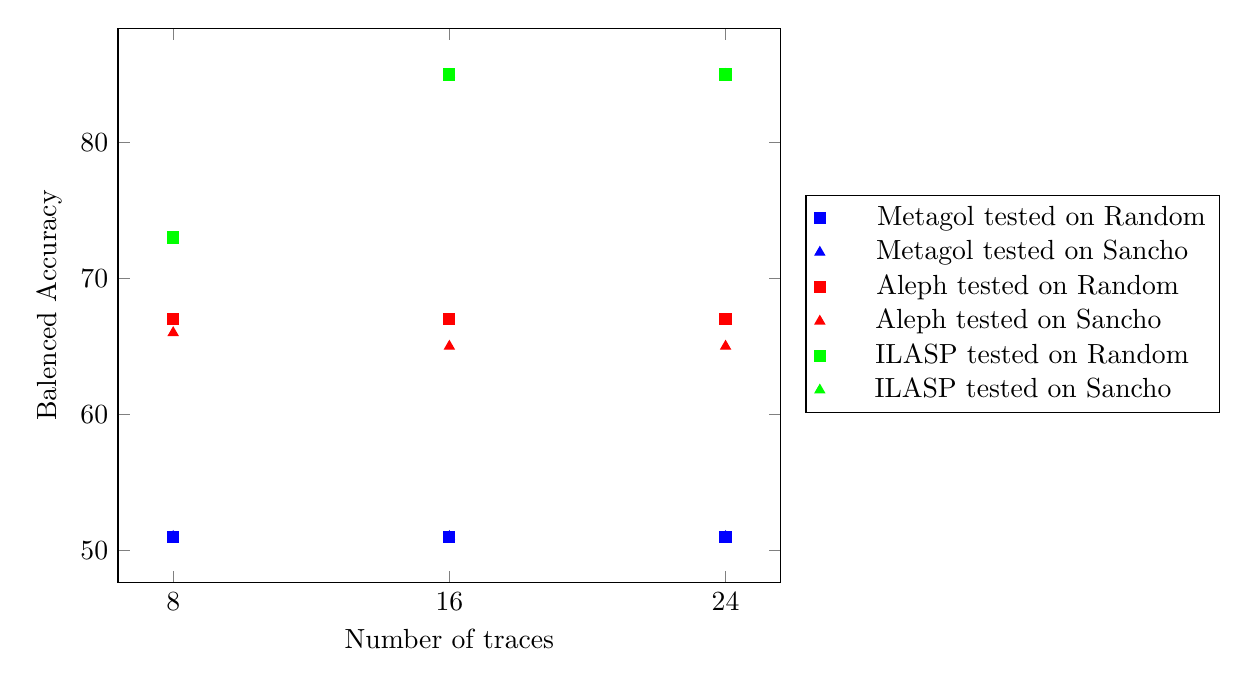
\begin{tikzpicture}
\begin{axis}[scatter/classes={
	a1={mark=square*,blue},%
	a2={mark=triangle*,blue},%
	b1={mark=square*,red},%
	b2={mark=triangle*,red},%
	c1={mark=square*,green},%
	c2={mark=triangle*,green}},
	legend style={at={(1.35,0.7)},
	anchor=north},
	xtick=data,
	ylabel={Balenced Accuracy},
	xlabel={Number of traces}]
\addplot[scatter,only marks,
	scatter src=explicit symbolic] coordinates {
	(8,51)     	[a1]
	(8,51)     	[a2]
	(16,51)    	[a1]
	(16,51)    	[a2]
	(24,51)    	[a1]
	(24,51)		[a2]
	(8,67)		[b1]
	(8,66)		[b2]
	(16,67)		[b1]
	(16,65)		[b2]
	(24,67)		[b1]
	(24,65)		[b2]
	(8,73)		[c1]
	(8,73)		[c2]
	(16,85)		[c1]
	(16,85)		[c2]
	(24,85)		[c1]
	(24,85)		[c2]
};
\legend{\ \ \ \ \ Metagol tested on Random,\ \ \ Metagol tested on Sancho,\ \ Aleph tested on Random,Aleph tested on Sancho, \ \ \ ILASP tested on Random,\ ILASP tested on Sancho,d}
\end{axis}

\end{tikzpicture}


%\subsubsection{Random training}
%\begin{tikzpicture}
%\begin{axis}[
%	ylabel=Balanced Accuracy,
%	width=6cm,
%	enlargelimits=0.05,
%	legend style={at={(0.5,1.3)},
%	anchor=north,
%	legend columns=-1},
%	ybar interval=0.5,
%	symbolic x coords={ilasp,metagol,aleph, poog}
%]
%\addplot
%	coordinates {(ilasp,71) (metagol,51) (aleph,66) (poog, 65)};
%\addplot
%	coordinates {(ilasp,72) (metagol,51) (aleph,65) (poog,65)};
%\legend{Tested on random,Tested on optimal}
%\end{axis}
%\end{tikzpicture}
%~
%\begin{tikzpicture}
%\begin{axis}[
%	width=6cm,
%	ylabel=Number of perfect games,
%	enlargelimits=0.05,
%	ybar interval=0.5,
%	symbolic x coords={ilasp,metagol,aleph, poog}
%]
%\addplot
%	coordinates {(ilasp,7) (metagol,0) (aleph,1) (poog, 0)};
%\addplot
%	coordinates {(ilasp,8) (metagol,0) (aleph,0) (poog,0)};
%\end{axis}
%\end{tikzpicture}
%\subsubsection{Optimal training}
%\begin{tikzpicture}
%\begin{axis}[
%ylabel=Balanced Accuracy,
%width=6cm,
%enlargelimits=0.05,
%legend style={at={(0.5,1.3)},
%	anchor=north,
%	legend columns=-1},
%ybar interval=0.5,
%symbolic x coords={ilasp,metagol,aleph, poog}
%]
%\addplot
%coordinates {(ilasp,71) (metagol,51) (aleph,65) (poog, 65)};
%\addplot
%coordinates {(ilasp,72) (metagol,51) (aleph,72) (poog,65)};
%\legend{Tested on random,Tested on optimal}
%\end{axis}
%\end{tikzpicture}
%~
%\begin{tikzpicture}
%\begin{axis}[
%width=6cm,
%ylabel=Number of perfect games,
%enlargelimits=0.05,
%ybar interval=0.5,
%symbolic x coords={ilasp,metagol,aleph, poog}
%]
%\addplot
%coordinates {(ilasp,5) (metagol,0) (aleph,0) (poog, 0)};
%\addplot
%coordinates {(ilasp,10) (metagol,0) (aleph,4) (poog,0)};
%\end{axis}
%\end{tikzpicture}


\chapter{Conclusions}
The benefits of training ILP systems to play games using human level and above gameplay traces verses random are negligible.

\af{describe what you did again, list limitations ("future work could"), paragraph for each limitation, what it is and how someone could address it}

\bibliography{project}
\bibliographystyle{plain}
\end{document}
